\documentclass{scrartcl}
\usepackage{style}
% version
\newcommand{\versionmajor}{0}
\newcommand{\versionminor}{1}
\newcommand{\versionpatch}{0}
\newcommand{\version}{\versionmajor.\versionminor.\versionpatch}
\usepackage{float}
\usepackage{subcaption}

\title{\LARGE
Intelligent Systems Engineering 2023/24 \newline
\newline
Literature survey: \\
Cybersecurity in Autonomous On-Road Motor Vehicles focusing on connectivity and perception systems
}

\author{
    Alberto Paganelli \\ \emailaddr{alberto.paganelli3@studio.unibo.it}
}

\date{\today}

\begin{document}

    \maketitle
    \begin{abstract}
    The rapid development of autonomous vehicles (AVs)
introduces transformative potential for modern transportation systems,
but it also raises critical concerns regarding cybersecurity.
As AVs increasingly rely on complexity, the attack surface for potential threats expands,
demanding robust and proactive security measures.
This survey aims to provide an overview of current research on security challenges in autonomous vehicles,
focusing on key cybersecurity threats, standards, and industry practices.
Emphasizing the need for a multi-layered approach to cybersecurity in AVs,
integrating secure software development, hardware resilience, and regulatory compliance is essential.
Moreover,
the survey explores future trends and emerging technologies that could enhance the security of autonomous vehicles helping the development of secure and reliable systems.
    \end{abstract}

    \newpage
    \tableofcontents
    \newpage

    \section{Methodology}\label{sec:methodology}
    \subsection{Premises}\label{subsec:premises}

In this review,
I aim to provide a comprehensive overview of the research current state on security in autonomous vehicles.
My focus is on the key cybersecurity threats, standards, and industry practices in the field,
keeping in mind that the landscape is rapidly evolving.
The goal is to identify the most critical challenges and opportunities for future research in this area
and underline the importance of a multi-layered approach to cybersecurity in AVs, starting from the design phase.
The ethical implications of the technology or the comparison between human-driven and autonomous vehicles in terms of accidents and fatalities will not be covered.

\subsection{Research Question}\label{subsec:research-question}

Starting from the main threats in terms of cybersecurity regarding AV, the review will analyze the main actual opportunities to improve and regulate the security of these systems.
After that, the review will focus on the industry practices concluding in the future trends and emerging technologies that could enhance and simplify the security process of AVs.
The goal of this review is to address the following research questions:

\begin{enumerate}
    \item \textit{What are the most significant cybersecurity threats facing autonomous vehicles, and how these threats evolve with advancements in vehicle-to-everything (V2X) communication and other emerging technologies?}
    \item \textit{What existing standards and regulatory frameworks govern cybersecurity by design in autonomous vehicles, and how effectively do they address current and future security challenges?}
    \item \textit{What cybersecurity solutions and practices have been implemented by autonomous vehicle manufacturers, and how do they align with best practices in secure software development and system resilience?}
    \item \textit{What future trends and emerging technologies, such as artificial intelligence and blockchain, are being explored to enhance the cybersecurity of autonomous vehicles?}
\end{enumerate}

\subsection{Selection Criteria}\label{subsec:selection-criteria}

The selection criteria for the literature review are as follows:
\begin{enumerate}
    \item \textit{Relevance:} The literature must be directly related to the topic of security in autonomous vehicles, focusing on cybersecurity threats, standards, and industry practices.
    \item \textit{Quality:} The literature should be published in reputable journals, conference proceedings, or books, ensuring high academic and technical standards.
    \item \textit{Recency:} The literature should be recent (published within the last five years) to reflect the latest developments in the field.
    \item \textit{Diversity:} The literature should cover a broad range of topics within the field of autonomous vehicle security, including but not limited to threat modeling, risk assessment, secure software development, and hardware security.
    \item \textit{Accessibility:} The literature should be accessible online or through academic libraries to ensure that it can be reviewed and cited effectively.
\end{enumerate}

Some references are not recent, but they are fundamental to understanding the historical context and the evolution of autonomous vehicles.

\subsection{Search Strategy}\label{subsec:search-strategy}

The search strategy for this review involved a systematic exploration of electronic databases, books, and relevant publications.
The following databases were used to identify relevant literature:

\begin{enumerate}
    \item Google Scholar
    \item IEEE Xplore
    \item WebOfScience
    \item SpringerLink
\end{enumerate}

Multiple searches were conducted, initially to discover in general the state of the art in the field of autonomous vehicles and then to focus on the security aspects.
The search terms used included combinations of the following keywords:
\textit{autonomous vehicles}, \textit{self-driving cars}, \textit{cybersecurity}, \textit{security threats}, \textit{standards}, \textit{industry practices}, \textit{V2X communication}, \textit{ISO/SAE 21434}, \textit{UNECE WP.29}, \textit{secure software development}, \textit{intrusion detection}, \textit{over-the-air updates}, \textit{encryption}, \textit{artificial intelligence}, \textit{digital twins} and \textit{blockchain}.

Some principal queries were:
\begin{enumerate}
    \item \textit{autonomous vehicles cybersecurity threats}
    \item \textit{autonomous vehicles cybersecurity standards}
    \item \textit{autonomous vehicles cybersecurity connectivity}
    \item \textit{autonomous vehicles cybersecurity perception sensors}
    \item \textit{autonomous vehicles cybersecurity architecture}
    \item \textit{autonomous vehicles cybersecurity accidents}
    \item \textit{autonomous vehicles cybersecurity V2V, V2I, V2X}
    \item \textit{autonomous vehicles cybersecurity TODO}
    \item \textit{autonomous vehicles cybersecurity future trends}
    \item \textit{secure software development lifecycle autonomous vehicle}
    \item \textit{autonomous vehicles secure over-the-air}
    \item \textit{autonomous vehicles cybersecurity future directions}
    \item \textit{autonomous vehicles cybersecurity privacy blockchain}
    \item \textit{autonomous vehicles cybersecurity artificial intelligence}
\end{enumerate}

Moreover, some filter was applied to search only recent results, only peer-reviewed articles, and only articles in English.
First, the search was conducted on IEEE Xplore and Google Scholar, and then the same search was replicated on the other databases to ensure the comprehensiveness of the results.

The search strategy aimed to identify a diverse range of sources, including academic papers, conference proceedings, books, and industry reports, to provide a comprehensive overview of research on security in autonomous vehicles.
In certain cases, the limit on the age of the publication was removed to include fundamental works that are not recent but representative of a specific technology or approach (think about CAN bus).
Moreover, some references are relative to the automotive industry in general, but they are fundamental to understanding the context in which autonomous vehicles are developed.

\subsubsection{Phases}\label{subsubsec:phases}
The search of papers and documents was conducted in two phases:
\begin{enumerate}
    \item \textit{General Search:} The initial search aimed to identify the main topics and subtopics related to security in autonomous vehicles.
    \item \textit{Focused Search:} The second search focused on specific aspects of cybersecurity in autonomous vehicles, such as threats, standards, industry practices, and future trend.
\end{enumerate}

Every search was conducted using the same keywords and filters.
To ensure consistency and comparability of results across different databases, in particular, the keywords \textit{autonomous vehicles} and \textit{cybersecurity} were always present in the search query to keep the focus on the main topic of the review.
Only for the~\ref{sec:future-directions} section, the year of publication was restricted to the last 2 years to ensure the most recent results and approaches.

In case of doubt about the relevance of a paper, the abstract was read to understand if the paper was pertinent to the topic of the review.
The number of citations was also considered but not like a primary filter, favoring instead the quality of the paper and the relevance in terms of cybersecurity of the content.


\subsection{Quality Assessment}\label{subsec:quality-assessment}
The quality assessment of the selected literature has been differentiated based on the type of citation.
For books, the evaluation has been based on the reputation of the author and the publisher, considering both their academic credentials and contributions to the field.
Additionally, the relevance of the book to the specific topics of cybersecurity and autonomous vehicles has been taken into account.

Given the interdisciplinary nature of this topic, papers from social sciences and related fields have also been included.
The grade of confidence for principal papers has been evaluated based on several factors: the demonstration of results, coherence of conclusions, and the methodology employed.
A rigorous methodology is essential for ensuring validity and reliability in research findings, as highlighted by [source 1] and [source 2].

Furthermore, peer-reviewed journal articles have been prioritized due to their critical review process, which enhances the credibility of the research.
Articles that provide empirical data or case studies have been weighted more heavily, as they offer concrete evidence to support theoretical claims.
The citation index and impact factor of journals have also been considered to gauge the influence of the research within the academic community.

In cases where studies span multiple disciplines, a qualitative analysis was conducted to assess the applicability of their findings to cybersecurity in autonomous vehicles.
This approach ensures a comprehensive understanding of the topic, acknowledging the complexity of cybersecurity challenges that intersect with social, ethical, and technological dimensions.


\subsection{Data Extraction}\label{subsec:data-extraction}

The data extraction process involved identifying key information from the selected literature to address the research questions.
The following data points were extracted from each source:
\begin{enumerate}
    \item \textit{Publication:} The title of the publication, including the journal, conference, or book where the work appeared.
    \item \textit{Year:} The publication year to determine the recency of the source.
    \item \textit{Research Focus:} A brief summary of the main research focus or objective of the publication.
    \item \textit{Key Findings:} The primary findings or results of the research, including any significant insights or conclusions.
    \item \textit{Methodology:} The research methodology employed in the study, such as case studies, surveys, experiments, or theoretical analysis.
    \item \textit{Relevance:} The relevance of the publication to the research questions and the broader topic of security in autonomous vehicles.
\end{enumerate}

\subsection{Limitations}\label{subsec:limitations}

The limitations of this review include the following:
\begin{enumerate}
    \item \textit{Scope:} The review focuses primarily on cybersecurity threats, standards, and industry practices in autonomous vehicles, excluding ethical, legal, and social implications.
    \item \textit{Recency:} Due to the rapidly evolving nature of the field, some of the literature may not capture the most recent developments in autonomous vehicle security.
    \item \textit{Accessibility:} The availability of certain publications may be limited, but access to academic databases and libraries minimized the issue.
    \item \textit{Interdisciplinary nature:} The interdisciplinary nature of the topic may present challenges in synthesizing findings from diverse fields, but efforts have been made to ensure a comprehensive and holistic review.
\end{enumerate}

\newpage


    \section{Introduction}\label{sec:introduction}
    The focus is on the security aspects of autonomous on-road motor vehicles,
in particular the cybersecurity threats, standards, and industry practices used to secure these systems.
The current state of the VANETs communication main technologies and sensors of the perception systems will be analyzed,
exploring the attack surface, main vulnerabilities and possible mitigations.

\subsection{Historical roots}\label{subsec:historical-roots}

The development of autonomous vehicles is a significant milestone in the evolution of intelligent transport systems.
It is important to start with some historical context to understand the current state of autonomous vehicles and then,
the security implications.

Vehicle automation has roots with General Motors showcasing the first concept of an automated vehicle in 1939.
Initial R\&D efforts were led by General Motors and the Radio Corporation of America Sarnoff Laboratory in the 1950s.
From 1964 to 2003, various government and academic initiatives in the US, Europe,
and Japan focused on automated buses, truck platoons, and advanced driving systems\cite{pendleton2017perception, shladover2017connected}.
A significant boost came from DARPA’s Grand Challenges Program in the 2000s\cite{darpa_grand_challenges_book},
where AVs first navigated desert terrains in 2005 and urban roads in 2007\cite{pendleton2017perception, shladover2017connected}.

Since then, researchers have rapidly progressed in academia and industry.
Volvo, Tesla, Audi, BMW,
Mercedes-Benz and Nissan are some of the major car manufacturers that have invested in AV technology\cite{faisal2019understanding}.

\begin{figure}[!htb]
    \centering
    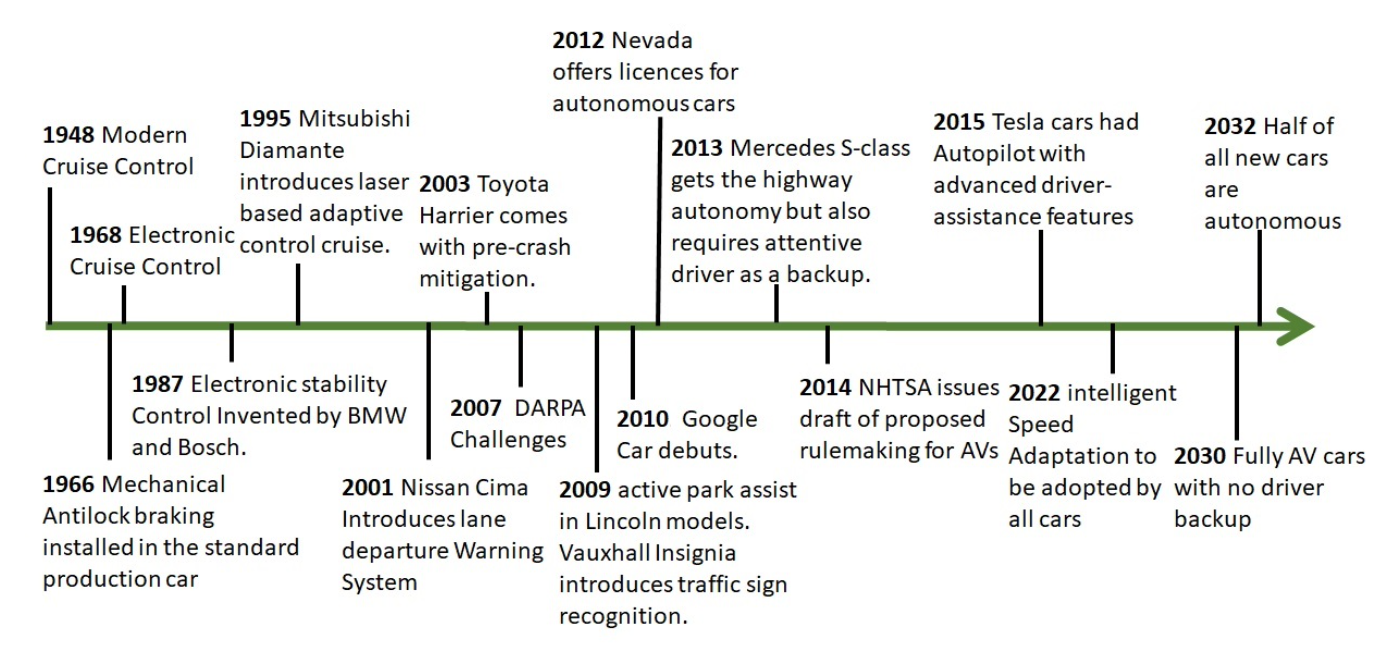
\includegraphics[width=0.7\linewidth]{figures/history}
    \caption{Historical timeline of autonomous vehicles.}
    \footnotesize{From \cite{ahangar2021survey} }
    \label{fig:history}
\end{figure}

\subsection{Autonomous Vehicles}\label{subsec:autonomous-vehicles}

The introduction on the market of autonomous vehicle brings to a revolutionary change in the automotive sector.
It is important to understand the impact that these vehicles can have on the society and the economy, influencing not only the automotive sector.
This type of vehicle can bring us to a new era of mobility, where transportation systems become intelligent, keeping in mind that connected components can be dangerous if not specially designed or well maintained\cite{schneier2014iot}

This major challenge, as often happens during times of innovation, has brought both advantages and drawbacks in terms of security.
What is intended is that the real driving force behind this innovation has been the convenience and socially beneficial aspects that have led to the rapid evolution of the sector.
However, as is often the case in such situations, some fundamental details get overlooked—it's a natural consequence.
In this instance, the principle of cybersecurity by design was overlooked\cite{sec-by-design}, and similar to the early development of the web, efforts are now underway to rectify this.

A lot of innovations also in terms of communication have been made since the introduction of these vehicles.
To improve functionalities, infotainment, safety, comfort and a lot of other aspects, vehicles require a lot of communication between them and the infrastructure like manufacturers backends or smart cities' services.
The shift from isolated and static systems to dynamic and interconnected systems increases the attack surfaces, particularly in terms of adaptability, dynamism, and awareness\cite{connected_vehicles_security_2023, bouchouia2023survey}.

For instance, vehicles relying on open software protocols and connecting with in-vehicle electric infrastructures play a vital role in strengthening their security framework.
With the need and integration of complex systems like the perception one, these vehicles essentially evolve into a highly sophisticated set of technologies influencing each other\cite{sec-by-design}.

\subsubsection{Levels of Automation}\label{subsubsec:levels-of-automation}
The level of driving automation is determined by the specific roles assigned to both the driving automation system feature and the human user in performing the dynamic driving task (DDT) and DDT fallback\cite{sae_j3016_2021}.
The manufacturer of the automation system defines the requirements, operational design domain (ODD), and operating characteristics of the feature, including its level of automation.
Additionally, the manufacturer outlines how the feature should be properly used, ensuring that its capabilities and limitations are clearly understood and followed during operation.
The Society of Automotive Engineers (SAE) has defined six levels of driving automation, ranging from no automation (Level 0) to full automation (Level 5)\cite{sae_j3016_2021}.

\begin{enumerate}
    \item \textbf{Level 0 (No Automation):} The human driver is responsible for all aspects of the dynamic driving task.
    \item \textbf{Level 1 (Driver Assistance):} The vehicle helps the driver with specific tasks, such as steering or acceleration (e.g.\ lane keeping assist, adaptive cruise control).
    \item \textbf{Level 2 (Partial Automation):} The vehicle can control both steering and acceleration/deceleration simultaneously under certain conditions, but the driver must remain engaged and monitor the environment (e.g. combined LKA and ADC in traffic conditions).
    \item \textbf{Level 3 (Conditional Automation):} The vehicle can perform all aspects of the DDT under certain conditions like in traffic jams or highway driving, but the driver must be ready to take over when prompted.
    \item \textbf{Level 4 (High Automation):} The user (become passenger) does not need to supervise the Automated driving system (ADS) or be receptive to a request to intervene while the
    ADS is engaged, restricted to some conditions (e.g., Google's Self-Driving Car\cite{teoh2017rage}).
    \item \textbf{Level 5 (Full Automation):} The vehicle can perform all aspects of the DDT under all conditions without human intervention.
\end{enumerate}

Levels 0–2 are generally classified as driver-assisted systems, while Levels 3 and 4 are considered semi-automated, and Level 5 represents full autonomy.

\begin{table}[ht]
    \centering
    \begin{tabular}{|c|l|}
        \hline
        \textbf{Acronym} & \textbf{Definition} \\ \hline
        ADS & Automated Driving System \\ \hline
        DDT & Dynamic Driving Task \\ \hline
        ODD & Operational Design Domain \\ \hline
        OEDR & Object and Event Detection and Response \\ \hline
    \end{tabular}
    \caption{Definitions of Key Acronyms in Automated Driving}
    \label{tab:acronyms}
\end{table}

\subsection{Overview of AVs Architecture}\label{subsec:overview-on-avs-architecture}

This section provides a high-level overview of the autonomous vehicles (AVs) architecture and the key parts that enable their operation.
Moreover, an alternative architecture proposed in\cite{ahangar2021survey} will be briefly discussed.
The architecture of AVs is designed to integrate various hardware and software components that work together to perceive the environment, make decisions, and control the vehicle\cite{architecture}.

\begin{figure}[!htb]
    \centering
    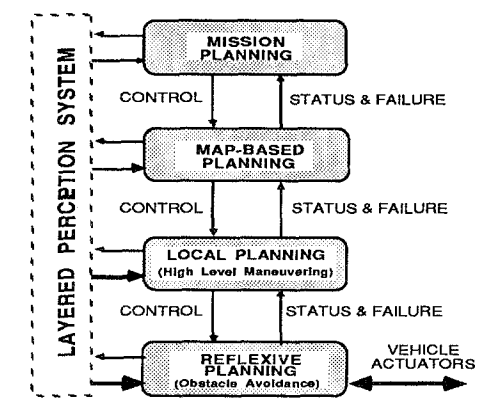
\includegraphics[width=0.7\linewidth]{figures/state-architecture}
    \caption{Hierarchical architecture of autonomous vehicles control.}
    \footnotesize{From \cite{architecture} }
    \label{fig:architecture}
\end{figure}

The overall architecture presented in\ref{fig:architecture} is composed of layers of hardware and software that interact to enable the vehicle to operate autonomously.
In its simplest and first form, the architecture consists of four main layers: perception, decision and planning, control and reflexive.
Each layer is responsible for a specific aspect of the AV's operation, from sensing the environment to executing driving maneuvers reflexively\cite{architecture}.

\begin{enumerate}
    \item \textbf{Perception}: This stage involves sensing the AV's surroundings using sensors.
    As expected, data processing is a fundamental step to exploit the correct information by other modules, such as adaptive detection and recognition frameworks, control systems, lane departure warning systems, traffic sign recognition, obstacle recognition, and vehicle positioning modules.
    The processed data is then sent to the decision and planning stage.
    It is important to note that performance in processing the data is fundamentals.
    \item \textbf{Decision and Planning}: Using the data from the perception stage, this stage plans and controls the AV's motion and behavior.
    It handles tasks like path planning, action prediction, and obstacle avoidance based on real-time maps, traffic data, user inputs, and past information.
    It may also include a data log module for error tracking and future reference.
    \item \textbf{Control}: The control module receives instructions from the decision and planning stage and manages the physical functions of the AV, such as steering, braking, and acceleration.
    \item \textbf{Reflexive}: This final stage interfaces with the mechanical components like the motors for the accelerator, brake, steering wheel, and gear.
    These components are controlled by the signals from the control module to execute the AV’s movements.
\end{enumerate}

The proposed and secured architecture extends this architecture providing four new layers: monitoring, analysis, decision-making, and visualization.
Any services, processes, and communication are monitored by the agents and analyzed by the process controllers.
A set of decision controllers act on the information from the process controllers.
The decisions are archived in a black box, while the analysis, reporting, and visualization layers are accessible both within the vehicle and through an external Virtual Security Operations Center (VSOC), allowing the user to consult them as needed\cite{adu-kyere2023self-aware}.

What can be easily noted is the need to monitor and analyze the data that are exchanged between the different components of the AVs.
Also, the data that are exchanged between the vehicle and the infrastructure should be monitored and analyzed to prevent and in case recover from possible attacks.
Some possible research directions could be the development of a secure and efficient monitoring system that can analyze the data in real-time and take action in case of attacks\ref{subsec:intrusion-detection-and-prevention-systems}.

\subsection{Social implications}\label{subsec:social-implications}

This section aims to provide a little insight into the social implications of autonomous vehicles.
The introduction of autonomous vehicles (AVs) is expected to have a profound impact on society\cite{thomas2020perception},
transforming transportation systems\cite{intelligent_transportation_2023}, urban planning\cite{impact_autonomous_vehicles_2018},
and the economy~\cite{economic_aspects_2020}.
Some potential pros and cons of AVs are summarized in Table~\ref{tab:table}.

\begin{table}[ht]
    \centering
    \begin{tabular}{|l|l|}
        \hline
        \textbf{Pros} & \textbf{Cons} \\ \hline
        Number of accidents reduced & Definition of legal responsibilities \\ \hline
        Time saved & Job losses \\ \hline
        Comfort & Price \\ \hline
    \end{tabular}
    \caption{Some pros and cons from \cite{ahangar2021survey} }\label{tab:table}
\end{table}

The consideration of time saved
is related to the trust that the user has in the vehicle and how effectively the cities in which the vehicles are used are designed and smart enough.
Some references to explore in depth the social implications are left above.

\subsection{Cyber-insecurity consequences}\label{subsec:cyber-insecurity}

Before introducing new threats of new autonomous vehicle technologies, it is important to understand some historical key attacks.
In the past, researchers have demonstrated various attacks on AVs, including remote hijacking, sensor spoofing, and data breaches.
The attack surface of AVs is expanding due to the increasing complexity of these systems, which rely on a combination of hardware, software, and communication technologies\cite{cybersec}.
This expansion is due to the aggressive attempts of manufacturers to
make vehicles fully autonomous in a short period of time and without considering the cybersecurity implications.
Focussing always on the functionalities offered to the driver in terms of comfort, the security of the vehicle has been considered as a secondary aspect, leading to a lot of vulnerabilities that can be exploited by attackers.

Some famous attacks that bring the attention to the cybersecurity of AVs are:
\begin{enumerate}
    \item The Jeep Cherokee hack in 2015: researchers remotely hijacked a Jeep Cherokee through its infotainment system, demonstrating the risks of cyber-attacks on connected vehicles\cite{miller2015remote}.
    \item The Tesla Model S hack in 2016: researchers exploited vulnerabilities in the vehicle's software to take control of the car's brakes, door locks, and other critical systems\cite{tesla_hack}.
    \item The Nissan Leaf hack in 2016: researchers demonstrated how an attacker could remotely control the vehicle's heating and air conditioning systems, drain the battery, and access the driver's personal information.
    \item The VW group hacked in 2016: researchers discovered vulnerabilities in the keyless entry systems of several VW group vehicles, allowing attackers to unlock the doors and start the engine without the key fob~\cite{garcia2016lock}.
    \item The Tesla cybertruck: it continues to be exploited by attackers to gain access to the vehicle's systems and control its functions remotely.
\end{enumerate}

These are only some examples of the risks associated with AVs and the need for robust cybersecurity measures to protect against cyber-attacks.

    \section{Cybersecurity Threats}\label{sec:cybersecurity-threats}
    In this section, the goal is to discuss potential threats about the two macro-areas covered by this report:
communication (specifically VANETs) and the perception system,
giving a comprehensive overview of the potential threats and the
countermeasures that can be adopted to mitigate them, focussing on remote attacks.
The multitude of technologies involved in these two areas makes the AVs vulnerable to a wide range of attacks,
decreasing the threshold of security.
With the threshold, it is meant the acceptable level of security that is needed to protect the system from attacks.
If not only the safety of the system but also the safety of other potential road users is taken into consideration,
the threshold must be extremely high.
Attackers can exploit vulnerabilities to compromise the safety and functionality of AVs,
posing significant risks to passengers, pedestrians, and other road users.
Since now cars are connected to the internet, there is no need to be physically close to the car to exploit these vulnerabilities and this expands the attack surface drastically.
In the past decade (2010 onward), nearly 79.6\% of all automotive attacks have been
remote attacks\cite{cybersec}.

\subsection{General}\label{subsec:communication-system}

This section highlights various attacks, possible tempering and threats that affect the security services in general regarding
the CIA triad.
It is important to mention that the CIA triad is a model designed to guide policies for information security, and in the list below, some techniques cannot be present.

\paragraph{Attack on Confidentiality}
\begin{enumerate}
    \item \textbf{Eavesdropping}: Intercepts confidential information, such as user identity and location.
    \item \textbf{Traffic Analysis}: Analyzes message transmission patterns to extract sensitive information.
    \item \textbf{Man-in-the-Middle}: Intercepts and alters messages between communicating vehicles.
    \item \textbf{Social Engineering}: Distracts and exploits drivers to gain access to confidential information.
    \item \textbf{Sybil Attack}: Uses multiple fake identities to mislead vehicles and compromise confidentiality.
    \item \textbf{GPS Spoofing}: Creates false GPS information, compromising location confidentiality.
\end{enumerate}

\paragraph{Attack on Data Integrity}
\begin{enumerate}
    \item \textbf{Masquerading}: Uses valid credentials to broadcast false messages.
    \item \textbf{Replay}: Repeats or delays transmissions, complicating emergency responses.
    \item \textbf{Message Tampering}: Modifies messages to influence driving behavior.
    \item \textbf{Illusion}: Generates misleading traffic warnings based on malicious data.
    \item \textbf{Node Impersonation}: Uses a valid user ID to impersonate another user, compromising the integrity of communications.
    \item \textbf{Key/Certificate Replication}: Uses duplicates to create confusion, affecting data authenticity and integrity.
\end{enumerate}

\paragraph{Attack on Availability}
\begin{enumerate}
    \item \textbf{Denial-of-Service}: Blocks vehicle communication, disrupting operations; can occur as distributed denial of service (DDoS)\cite{sontakke2022impact}.
    \item \textbf{Jamming}: Uses strong signals to disrupt communication channels, critical for safety applications.
    \item \textbf{Malware}: Penetrates OBUs, RSUs or other system component leading to system malfunctions.
    \item \textbf{Broadcast Tampering}: Untrustworthy vehicles alter or replicate messages, hiding critical safety information.
    \item \textbf{Black-hole}: Malicious nodes receive but do not forward packets, obstructing communication.
    Another version is the \textit{Gray-hole} that selectively drops only some packets.
\end{enumerate}


To deepen the knowledge about other specific techniques for attacking and potential countermeasures, a specific evaluation
can be found in~\cite{simulation-attacks-vanets, sheikh2019comprehensive, macena2023cybersecurity}.

\begin{table}[h]
    \centering
    \begin{tabular}{|l|l|l|}
        \hline
        \textbf{Attack} & \textbf{Compromised} & \textbf{Countermeasures} \\ \hline
        DOS & A & Signature-based authentication technique \ref{subsec:intrusion-detection-and-prevention-systems} \\ \hline
        Jamming & A & Direct-sequence spread spectrum (DSSS\cite{wang2022when}) \\ \hline
        Malware & A & Reliable hardware and digital signature of software \\ \hline
        Broadcast tampering & I, A & Non-repudiation mechanism may exist \\ \hline
        Black-hole, gray-hole & A & Reliable hardware and digital signature of software \\ \hline
        Greedy behavior & A & Use intrusion detection systems (IDSs) \\ \hline
        Spamming & C, A & Reliable hardware and digital signature of software \\ \hline
        Eavesdropping & C, I & Exploit physical layer security protocols \\ \hline
        Traffic analysis & C & Encryption techniques \\ \hline
        Man-in-the-middle & C, I, A & Robust authentication technique (E.g. CA) \\ \hline
    \end{tabular}
    \label{tab:Summary of Attacks and Countermeasures}
\end{table}
A = Availability, AU = Authentication, C = Confidentiality, I = Integrity
from\cite{sheikh2019comprehensive}.

\subsection{VANETs}\label{subsec:v2x-communication-and-network}

In this section, the focus is on the communication system, specifically on the VANETs.
Some countermeasures are presented to mitigate the threats that affect the security services in VANETs, in particular the location privacy and related info.
Some of the main countermeasures, with benefits and limitations, are presented and discussed.

\subsubsection{Pseudonym Change and Silent Periods}
Dividing road networks into observed and unobserved zones allow vehicles to change pseudonyms and behavior, such as altering speeds and directions in unobserved zones.
This, combined with random silent periods in vehicle-to-vehicle (V2V) communication, reduces the risk of tracking and identity linking.
However, this technique can lead to privacy loss and computational strain for certain vehicles, particularly in V2I (vehicle-to-infrastructure) interactions, where more complex tasks are required.

\begin{enumerate}
    \item \textbf{Key Features}:
    \begin{enumerate}
        \item Road networks divided into observed/unobserved zones.
        \item Vehicles in unobserved zones change pseudonyms, directions, and speeds.
        \item Random silent periods in V2V communications to unlink identities.
    \end{enumerate}
    \item \textbf{Limitations}: Navigation group leaders privacy and computational overhead in V2I applications.
\end{enumerate}

\subsubsection{Cryptographic MIX-Zone (CMIX)}
Here, RSUs (Roadside Units) provide cryptographic keys to vehicles, enabling secure pseudonym exchanges in encrypted zones.
This method strengthens privacy, but the high costs of the required hardware and the complexity of managing pseudonym certification represent significant hurdles, particularly when applied on a larger scale.
\begin{enumerate}
    \item \textbf{Key Features}:
    \begin{enumerate}
        \item RSUs provide vehicles with cryptographic keys.
        \item Pseudonym exchange in encrypted mixing zones.
        \item Possible pseudonym certification through authorities.
        \item Optional use of hardware security modules (HSMs).
    \end{enumerate}
    \item \textbf{Challenges}: High hardware costs and managing pseudonym certification.
\end{enumerate}

\subsubsection{K-Anonymity}
A trusted server anonymizes data, and location information is shared only if enough vehicles are present nearby, making individual tracking more difficult.
This technique is scalable and can be adjusted based on vehicle density, making it well-suited for dynamic traffic conditions.
\begin{enumerate}
    \item \textbf{Key Features}:
    \begin{enumerate}
        \item Trusted server anonymizes data via cloaking.
        \item Location shared only if \emph{K} vehicles are nearby.
    \end{enumerate}
    \item \textbf{Advantages}: Scalable and customizable based on vehicle density.
\end{enumerate}

\subsubsection{Dynamically Changing MAC/PHY}
Periodic swapping of these addresses complicates tracking efforts.
Cryptographic key exchanges ensure that address changes are secure, although this approach requires careful management of the cryptographic process to maintain seamless communication.
\begin{enumerate}
    \item \textbf{Key Features}:
    \begin{enumerate}
        \item Periodic MAC/PHY address swapping.
        \item Cryptographic key exchange during address changes.
    \end{enumerate}
    \item \textbf{Advantages}: Makes vehicle tracking harder.
\end{enumerate}

\subsubsection{Density-Based Location Privacy (DLP)}
Offers protection by changing pseudonyms based on the number of surrounding vehicles.
In high-traffic areas, this method enhances privacy, but determining the optimal conditions for triggering pseudonym changes can be a challenge,
particularly in environments with rapidly shifting traffic densities.
\begin{enumerate}
    \item \textbf{Key Features}:
    \begin{enumerate}
        \item Pseudonym change occurs with \emph{k} neighboring nodes.
        \item Improved privacy in high-traffic areas.
    \end{enumerate}
    \item \textbf{Challenges}: Dynamic pseudonym change thresholds.
\end{enumerate}

The integration of pseudonyms, cryptographic techniques, dynamic address changes, and density-based strategies offers a comprehensive framework
for improving location privacy, however, practical implementation requires careful consideration of the associated costs and complexities\cite{macena2023cybersecurity}.


\subsection{Perception System}\label{subsec:perception-system}

The perception system in AVs is responsible for collecting and processing data from various sensors to understand the vehicle's surroundings.
The data collected by the perception system is crucial for making informed decisions and coordinating the vehicle's actuators in a safe and efficient manner.
However, since it is composed by a multitude of sensors, the perception system is a subsystem where the attack surface is huge\ref{fig:sensors-2}.
In this section, some main issues about the perception system will be presented and discussed, focusing on the potential threats and the countermeasures that can be adopted to mitigate them\cite{sensors}.

As mentioned, some sensors are \textit{LiDAR}, \textit{radar}, \textit{cameras}, and \textit{ultrasonic sensors}, to perceive and interpret their surroundings accurately.
For their nature, it is challenging preventing from common attacks like spoofing and jamming.
Sensor spoofing involves introducing false data into the sensor systems, while jamming overwhelms the sensors with noise, disrupting their normal functioning.

Through such manipulation, attackers can deceive the vehicle's control systems, causing misinterpretations of the environment.
For example, projecting fake obstacles might cause unnecessary breaking, while concealing real obstacles could lead to collisions.
These manipulations result in erratic driving behavior.
In cases of jamming, AVs may become \textit{careless} to their surroundings, resulting in dangerous situations due to the absence of reliable sensor input\cite{durlik2022cybersecurity}.

\begin{figure}[!htb]
    \centering
    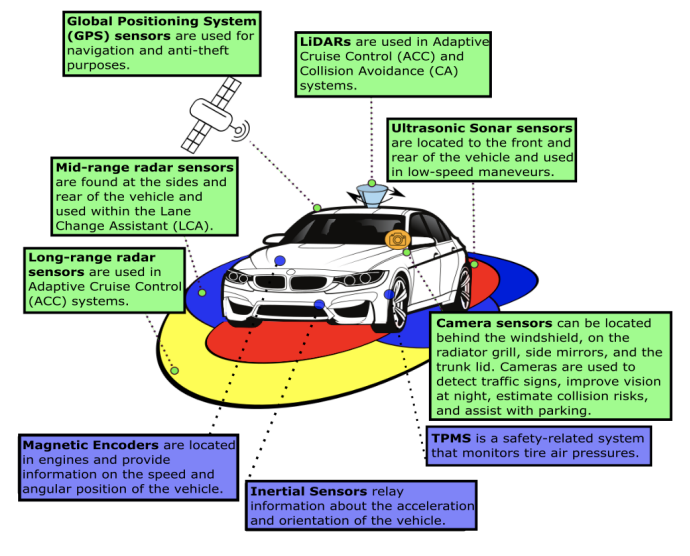
\includegraphics[width=0.7\linewidth]{figures/sensors}
    \caption{Main sensors used in AVs from \cite{sensors}}
    \label{fig:sensors-2}
\end{figure}

What emerges from the literature is that the perception system is a critical component of AVs, mainly every sensor can be a potential target for cyber-attacks using the techniques mentioned above.
From LiDAR, Ultrasonic Sensor, Camera, Radar, GPS, that are the most common sensors used is AVs, to the Tire Pressure sensors are all potential targets\cite{sensors}.


\paragraph{Countermeasures}

Given the complexity of autonomous vehicle perception systems, they can easily become a target for attacks.
The current approach acknowledges this vulnerability, which is challenging to fully eliminate.
Instead, the focus is shifting towards recognizing the stimuli detected by these systems and determining whether they are legitimate or not.
As highlighted in the machine learning/AI section\ref{subsec:artificial-intelligence}, machine learning algorithms—particularly those for anomaly detection—are being employed to identify and respond to irregularities in sensor data.
Another possible countermeasure is sensor fusion, which involves cross-referencing data from multiple sensors.
This technique helps to provide more accurate measurements and enables more stable decision-making and reactions.

However, while machine learning offers new avenues for detecting and mitigating these attacks, it introduces new challenges in terms of legal and ethical considerations.
Since the focus is not on these aspects but in the technical ones, it is essential to consider the forensic implications
of these algorithms\cite{durlik2022cybersecurity, cybersecurity2022forensics} and possible research for the future to eliminate these vulnerabilities.

\begin{figure}[!htb]
    \centering
    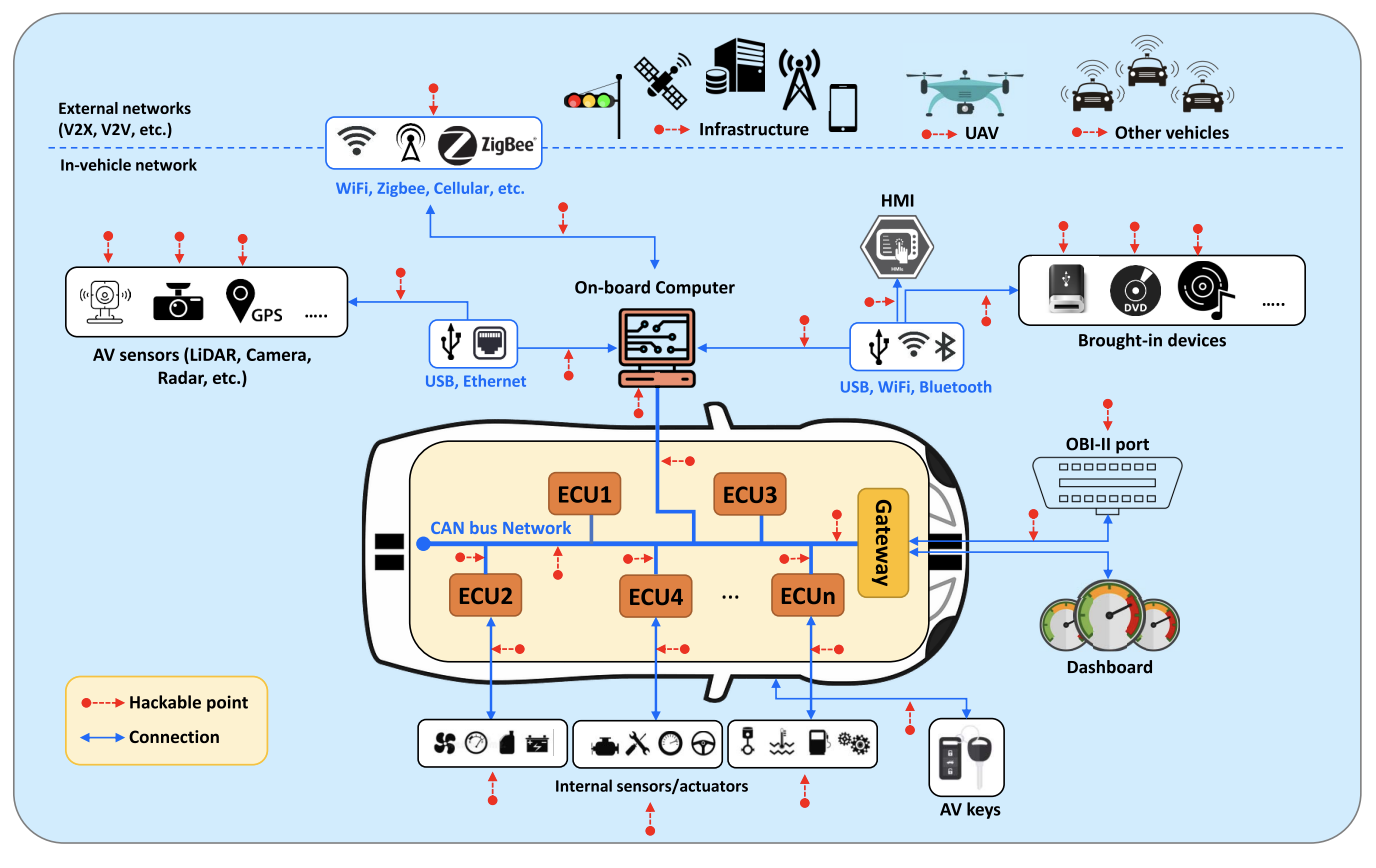
\includegraphics[width=0.7\linewidth]{figures/vectors}
    \caption{Main attack vectors from \cite{bendiab2023autonomous}}
    \label{fig:attack-vectors}
\end{figure}

    \section{Cybersecurity by design standards}\label{sec:cybersecurity-by-design-standards}
    \subsection{ISO/SAE 21434: Overview}\label{subsec:iso-sae-21434}
\href{url}{text}

The ISO/SAE 21434 standard is a joint standard
developed by the \href{https://www.iso.org/home.html}{International Organization for Standardization (ISO)} and the
\href{https://www.sae.org/}{Society of Automotive Engineers (SAE)} to address the cybersecurity of road vehicles.
The standard is designed to provide a framework for the development of secure vehicles and their components.
The standard covers the entire lifecycle of a vehicle, from design and development to production and operation.
It provides guidelines for identifying and assessing cybersecurity risks, as well as for implementing security measures to mitigate those risks.
The standard also includes requirements for monitoring and responding to cybersecurity incidents, as well as for managing the security of vehicle components and systems.
The ISO/SAE 21434 standard is intended to be used by vehicle manufacturers,
suppliers, and other stakeholders in the automotive industry to improve the cybersecurity of vehicles and protect them from cyber threats\cite{iso-correlation}.

\textbf{ISO/SAE 21434} is the international standard designed to address cybersecurity in road vehicles, particularly focusing on electrical and electronic (E/E) systems.
Released in August 2021, this standard establishes guidelines for original equipment manufacturers (OEMs) and suppliers to manage cybersecurity risks throughout the entire lifecycle of vehicle systems.
Moreover, it introduces the concept of Cybersecurity Assurance Levels, which categorize the severity of cybersecurity threats and the corresponding measures to mitigate them\cite{moukahal2021towards}.
\subsubsection{Key Points}\label{subsubsec:key-points-1}

\begin{enumerate}
    \item \textbf{Cybersecurity Culture}:
    \begin{enumerate}
        \item Promotes a strong cybersecurity culture within organizations, emphasizing safety and security in all engineering processes.
    \end{enumerate}

    \item \textbf{Risk Management}:
    \begin{enumerate}
        \item Provides guidelines for identifying and managing cybersecurity risks, including threat analysis, impact assessment, and risk mitigation strategies.
    \end{enumerate}

    \item \textbf{Documentation Requirements}:
    \begin{enumerate}
        \item Establishes a series of required work products, including asset identification, threat scenarios, and a cybersecurity incident response plan.
    \end{enumerate}

    \item \textbf{Lifecycle Integration}:
    \begin{enumerate}
        \item Covers cybersecurity from the initial design phase to decommissioning, ensuring that security measures are integrated throughout the vehicle's lifecycle.
    \end{enumerate}

    \item \textbf{Collaboration with Other Standards}:
    \begin{enumerate}
        \item Works in conjunction with existing standards, particularly ISO 26262 (which focuses on functional safety), ensuring that both safety and security are considered during vehicle development.
    \end{enumerate}

    \item \textbf{Continuous Monitoring and Improvement}:
    \begin{enumerate}
        \item Encourages continuous cybersecurity assessment and updates to address evolving threats and vulnerabilities.
    \end{enumerate}
\end{enumerate}

\subsubsection{Correlations}\label{subsubsec:correlations}

\begin{enumerate}
    \item \textbf{ISO 26262}: Emphasizes the relationship between safety and cybersecurity, ensuring that both aspects are addressed in vehicle design.
    \item \textbf{UNECE WP.29 R155}: Provides a legal framework for cybersecurity in vehicles, complementing ISO/SAE 21434 by outlining regulatory requirements and compliance timelines.
\end{enumerate}

\subsubsection{Limitations}\label{subsubsec:limitations}

\begin{enumerate}
    \item \textbf{Lack of Specific Technical Solutions}:
    \begin{enumerate}
        \item The standard does not prescribe specific technologies or methods for implementing cybersecurity measures, potentially leading to varied interpretations and implementations among manufacturers.
    \end{enumerate}

    \item \textbf{Potential for Fragmentation}:
    \begin{enumerate}
        \item Without defined methods, companies may adopt proprietary solutions that could create compatibility issues within a highly connected automotive environment.
    \end{enumerate}

    \item \textbf{No Mandatory Compliance}:
    \begin{enumerate}
        \item ISO/SAE 21434 is a guideline rather than a regulation, meaning compliance is not enforced by law, which could lead to inconsistent application across the industry.
    \end{enumerate}

    \item \textbf{Limited Focus on Cybersecurity Techniques}:
    \begin{enumerate}
        \item While the standard outlines processes and documentation, it does not provide detailed methodologies for specific cybersecurity assessments or techniques to evaluate vulnerabilities effectively.
    \end{enumerate}
\end{enumerate}

\subsubsection{Guidelines and countermeasure}\label{subsubsec:guidelines-and-countermeasure}

\begin{enumerate}
    \item \textbf{Threat Analysis and Risk Assessment}:
    \begin{enumerate}
        \item The standard emphasizes conducting thorough threat assessments to identify potential vulnerabilities in vehicle systems and the likelihood of cyberattacks.
    \end{enumerate}

    \item \textbf{Incident Response}:
    \begin{enumerate}
        \item Requires the establishment of a cybersecurity incident response plan to ensure quick and effective actions are taken in the event of a security breach.
    \end{enumerate}

    \item \textbf{Continuous Improvement}:
    \begin{enumerate}
        \item Advocates for regular updates and improvements to cybersecurity practices to adapt to new and emerging threats in the automotive landscape.
    \end{enumerate}
\end{enumerate}

\subsubsection{Conclusion}\label{subsubsec:conclusion}

ISO/SAE 21434 aims to enhance the cybersecurity posture of the automotive industry by establishing a comprehensive framework for managing risks associated with E/E systems in vehicles.
While it addresses critical aspects of cybersecurity, its limitations, particularly the lack of prescribed technical solutions and mandatory compliance, highlight the need for continued development and adaptation to effectively mitigate evolving cybersecurity threats.

\subsection{UNECE WP.29: Overview}\label{subsec:unece-wp-29}

The United Nations Economic Commission for Europe (UNECE) oversees regulations concerning cybersecurity and software updates for road vehicles, specifically through the UNECE WP.29 framework.

\subsubsection{Key Points}\label{subsubsec:key-points}
\begin{enumerate}
    \item \textbf{Cybersecurity Regulations (R155)}: Established in March 2021, these regulations are crucial for OEMs and Tier suppliers in UNECE member countries.
    Compliance is mandatory for new vehicle types since July 2022 and for all vehicles from July 2024.
    \item \textbf{Components of R155}:
    \begin{enumerate}
        \item \textbf{Cybersecurity Management System (CSMS)}: Organizations must implement a CSMS to manage cyber risks across the vehicle lifecycle.
        This systematic approach involves defining processes, responsibilities, and governance to protect vehicles from cyber threats.
        \item \textbf{Certification}: OEMs must apply for a Certificate of Compliance for their CSMS, which is valid for three years, subject to renewal.
        The approval process involves assessments and validation by technical services and Approval Authorities.
    \end{enumerate}
\end{enumerate}

\subsubsection{Threats and Mitigations in R155}\label{subsubsec:threats-and-mitigations-in-r155}
\begin{enumerate}
    \item \textbf{Annex 5 Structure}:
    \begin{enumerate}
        \item \textbf{Part A}: Identifies 32 potential threats related to various attack surfaces (e.g., communication channels, back-end servers).
        Each threat includes examples of vulnerabilities affecting Confidentiality, Integrity, and Availability (CIA) of vehicle systems.
        \begin{enumerate}
            \item \textbf{Confidentiality Threats}: For example, eavesdropping on communications.
            \item \textbf{Integrity Threats}: Unauthorized manipulation or deletion of vehicle data.
            \item \textbf{Availability Threats}: Risks such as Denial of Service (DoS) attacks that may compromise user safety.
        \end{enumerate}

        \item \textbf{Part B}: Outlines high-level mitigation actions specifically for vehicle-related threats.
        For instance, to protect confidential data in transit, one suggested mitigation is to ensure that all confidential communications are safeguarded, although it does not detail specific implementations.

        \item \textbf{Part C}: Addresses threats from external entities, such as back-end servers.
        It recommends measures like applying security checks and adhering to OWASP guidelines to prevent unauthorized access.
    \end{enumerate}
\end{enumerate}

Overall, the UNECE regulations emphasize a comprehensive and systematic approach to cybersecurity in the automotive sector, requiring OEMs to be proactive in identifying risks and implementing suitable mitigations.


\subsection{Comparative Analysis}\label{subsec:comparative-analysis}
\begin{figure}[!htb]
    \centering
    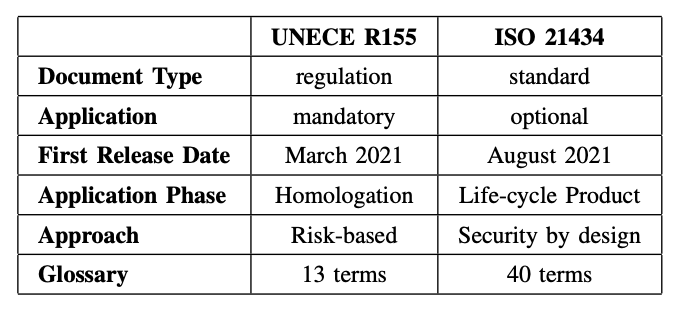
\includegraphics[width=0.7\linewidth]{figures/diff-standards}
    \caption{Comparison of ISO/SAE 21434 and UNECE WP.29 R155}
    \footnotesize{From \cite{comparison-standard} }
    \label{fig:comparison}
\end{figure}

The development of UNECE R155 and ISO/SAE 21434 arose from the need to enhance cybersecurity in road vehicles to ensure user safety and protect personal data.
Although UNECE R155 was released in March 2021 and ISO/SAE 21434 followed in August 2021, the two documents serve different purposes within the automotive cybersecurity landscape.
Here’s a detailed analysis of their similarities, differences, and limitations.

\subsubsection{Similarities}

\begin{enumerate}
    \item \textbf{Common Objectives}: Both UNECE R155 and ISO/SAE 21434 aim to improve cybersecurity throughout the product lifecycle of road vehicles, enhancing user safety and data protection.

    \item \textbf{High-Level Solutions}: Both documents propose high-level solutions and do not prescribe specific implementations, allowing manufacturer flexibility to adopt suitable measures for their contexts.
    \begin{enumerate}
        \item \textbf{Threat Identification}: UNECE R155 identifies possible threats, such as malicious internal messages, while ISO/SAE 21434 cites similar scenarios requiring analysis and mitigation.
    \end{enumerate}

    \item \textbf{Structured Organization}: Both documents require a structured approach to managing cybersecurity, including
    \begin{enumerate}
        \item Cybersecurity Management Systems (CSMS) and risk identification.
        \item Continuous monitoring and improvements, supported by internal or external audits.
    \end{enumerate}

    \item \textbf{Risk Mitigation}: Both documents emphasize risk mitigation processes, where UNECE R155 focuses on risk management and ISO/SAE 21434 outlines specific risk treatment options (e.g., avoiding, reducing, sharing).

    \item \textbf{Documentation for Compliance}: Documentation required for ISO/SAE 21434 can support compliance with UNECE R155, facilitating a cohesive approach to managing cybersecurity.

    \item \textbf{Continuous Review}: Both documents mandate the ongoing revision of cybersecurity practices and documentation throughout the vehicle lifecycle, ensuring ongoing support and updates.

    \item \textbf{Cost Considerations}: Both UNECE R155 and ISO/SAE 21434 acknowledge the need for cybersecurity compliance that balances implementation costs with operational feasibility, highlighting the complexity of the automotive environment.
\end{enumerate}

\subsubsection{Differences}

\begin{enumerate}
    \item \textbf{Type of Document}:
    \begin{enumerate}
        \item \textbf{UNECE R155}: A legally binding regulation that mandates compliance for all UNECE member countries.
        \item \textbf{ISO/SAE 21434}: A non-mandatory standard expected to be widely accepted within the automotive industry.
    \end{enumerate}

    \item \textbf{Implementation Timeline}:
    \begin{enumerate}
        \item \textbf{UNECE R155}: Compliance was mandated for new vehicle types from July 2022 and for all vehicles by July 2024.
        \item \textbf{ISO/SAE 21434}: Became applicable from August 2021.
    \end{enumerate}

    \item \textbf{Application Phases}:
    \begin{enumerate}
        \item \textbf{UNECE R155}: Focused primarily on the homogenization phase, requiring documentation for getting a Certificate of Compliance for the CSMS.
        \item \textbf{ISO/SAE 21434}: Encompasses the entire product lifecycle, requiring ongoing documentation for annual audits, from design to decommissioning.
    \end{enumerate}

    \item \textbf{Glossary Size}:
    \begin{enumerate}
        \item \textbf{ISO/SAE 21434}: Contains a comprehensive glossary with over three times more definitions than UNECE R155, which aids in clarity and understanding of cybersecurity terminology.
        \item \textbf{UNECE R155}: Lacks detailed definitions, potentially leading to varied interpretations of terms like \textit{confidential data}.
    \end{enumerate}

    \item \textbf{Threat and Mitigation Approach}:
    \begin{enumerate}
        \item \textbf{UNECE R155}: Provides tables outlining specific threats and recommended mitigations.
        \item \textbf{ISO/SAE 21434}: Does not directly address attacks but emphasizes vulnerability analysis and risk assessments.
    \end{enumerate}

    \item \textbf{Detail of Compliance Requirements}:
    \begin{enumerate}
        \item \textbf{UNECE R155}: Offers a less detailed list of compliance documentation compared to ISO/SAE 21434, which specifies required work products in detail.
        \item \textbf{ISO/SAE 21434}: Details the attack feasibility ratings and their implications in Annex G, emphasizing the importance of selecting appropriate methods for risk-based decisions.
    \end{enumerate}

    \item \textbf{Regulatory Authority}:
    \begin{enumerate}
        \item \textbf{UNECE R155}: Enforced by regulatory authorities in UNECE member states, with compliance being mandatory.
        \item \textbf{ISO/SAE 21434}: Lacks mandatory enforcement, relying on industry acceptance and best practices.
    \end{enumerate}
\end{enumerate}

\subsubsection{Conclusion}\label{subsubsec:conclusion2}

In conclusion, while UNECE R155 and ISO/SAE 21434 share common goals of enhancing cybersecurity in the automotive industry, they differ significantly in their nature, application, and requirements.
UNECE R155 is a binding regulation focused on approval, while ISO/SAE 21434 serves as a comprehensive standard for the entire vehicle lifecycle.
Their complementary nature allows manufacturers to leverage the documentation and processes of one to meet the requirements of the other,
fostering a more robust approach to cybersecurity in road vehicles\cite{comparison-standard}.
The problem remains that the lack of mandatory enforcement in ISO/SAE 21434 could lead to inconsistent implementation across the industry and potentially undermine the standard's effectiveness in addressing cybersecurity threats.

    \section{Actual Solutions}\label{sec:actual-solutions}
    \subsection{Secure Software Development Life-Cycle}\label{subsec:secure-software-development-life-cycle}

Cybersecurity in autonomous vehicles (AVs) is a critical concern that requires a comprehensive and multi-faceted approach.
One of the key strategies for enhancing AV security is the implementation of secure software development practices.
The secure software development life cycle (SDLC) is a systematic and structured approach to developing software that prioritizes security at every stage of the development process.
By integrating security considerations into the software development process from the outset, developers can identify and mitigate security vulnerabilities early, reducing the risk of cyberattacks and data breaches.
To maintain the security of the software in AVs, a specific way to update the software is needed\ref{subsubsec:secure-over-the-air-ota-updates}.

The major challenges in implementing a secure software development life-cycle are the
\begin{enumerate}
    \item \textbf{Complexity of AV Systems}: AV systems are complex and interconnected, containing a huge number of LOC that can easily introduce vulnerabilities.
    \item \textbf{Various Technologies}: AV systems are composed of various technologies, including sensors, actuators, and communication systems, each of which presents unique security challenges in terms of code vulnerabilities and attack surfaces.
    \item \textbf{Outsourcing}: Many AV manufacturers outsource software development to third-party vendors, introducing possible supply chain vulnerabilities.
    \item \textbf{Open-source Code}: This can be a source of vulnerabilities if not properly managed.
    \item \textbf{Security Decays Over Time}: As software ages, vulnerabilities may be discovered, and security patches may be required.
\end{enumerate}

To address these challenges, AV manufacturers must adopt a security-first mindset and integrate security into every phase of the software development life cycle\cite{moukahal2021towards}.
The main phases of the secure software development life cycle include:

\begin{enumerate}
    \item \textbf{Requirement Analysis:} Consider the complexity of automotive systems that require special security consideration to manage it properly.
    \item \textbf{Design:} Examine the system architecture thoroughly to construct proper measures limiting system weaknesses.
    \item \textbf{Assurance Planning:} Guarantees that manufacturers are ready to take proper and prompt actions to mitigate cyber incidents, starting after the cybersecurity Design phase to ensure incident response planning abides by the system design.
    \item \textbf{Implementation:} Involves security engineers monitoring the development of automotive components to confirm compliance with secure coding practices.
    \item \textbf{Component Testing:} Part of the security verification phases dedicated to ensuring the integrity of individual components.
    \item \textbf{Integration Testing:} Evaluates the interactions between integrated components to identify potential vulnerabilities.
    \item \textbf{Resilience Verification:} Assesses the overall resilience of the system against cyber threats.
\end{enumerate}

In conclusion, the cybersecurity challenge requires a comprehensive and multi-faceted approach, and the secure software development life cycle is a key strategy for enhancing AV security.

\subsection{Intrusion Detection and Prevention Systems}\label{subsec:intrusion-detection-and-prevention-systems}
IDPS are essential components of a comprehensive cybersecurity strategy for AVs, they allow for real-time monitoring and detection of potential cyber threats, enabling rapid response and mitigation of security incidents.
As mentioned in\cite{kim2020cybersecurity} the need of an intrusion detection system is not something new, research papers have been published since 2009, and the need for a proper system is still present.

Before the emergence of connected vehicles, the primary emphasis was on detecting malicious software within the vehicle itself.
However, the focus has now expanded to include a broader range of threats beyond just in-vehicle malware detection.
This type of systems helps to detect and prevent unauthorized access to the vehicle's network, monitor the behavior of connected devices, and identify anomalous activities that may indicate a cyberattack.
New approaches make large use of machine learning algorithms to detect anomalies in the vehicle's network traffic, and to identify patterns that may indicate a potential security threat\cite{nagarajan2023machine}.

\subsubsection{Secure Over-the-Air (OTA) Updates}\label{subsubsec:secure-over-the-air-ota-updates}

One of the key challenges in maintaining the security of AVs is the need to update software and firmware over-the-air (OTA) to address security vulnerabilities and bugs.
Over-the-air (OTA) updates are crucial for maintaining both the security and functionality of autonomous vehicle (AV) systems\cite{durlik2022cybersecurity, ahangar2021survey}.
Secure OTA mechanisms ensure that software updates are properly authenticated and delivered without the risk of tampering.

OTA updates will facilitate rapid software distribution and bug fixes for the embedded software on electronic control units.
However, in terms of security, OTA updates pose significant challenges due to their complexity, multiple attack surfaces, and reliance on outdated techniques.

Some main functionalities of OTA updates are:
\begin{enumerate}
    \item \textbf{Addressing Vulnerabilities}: Rapid hot-fix security of flaws reducing the risk of exploitation.
    \item \textbf{Enhancing Security Features}: Patching intrusion detection and authentication protocols.
    \item \textbf{Bug Fixes}: Resolving software bugs that may cause malfunctions or security risks.
    \item \textbf{Adapting to Emerging Threats}: Updating software to counter new and evolving cybersecurity threats.
    \item \textbf{Minimizing Downtime}: Ensuring updates occur with minimal disruption to vehicle operation.
    \item \textbf{Maintaining Compliance}: Keeping the vehicle up to date with regulatory security standards.
\end{enumerate}

\textbf{Best practices}:
\begin{enumerate}
    \item \textbf{Secure Update Mechanism}: Ensures the integrity and confidentiality of the update process through authentication and encryption.
    \item \textbf{Testing and Validation}: Rigorous testing to prevent new vulnerabilities and maintain functionality.
    \item \textbf{User Notification and Consent}: Informing users about updates and getting consent when necessary.
    \item \textbf{Regular Update Schedule}: Consistent schedule to ensure timely updates.
\end{enumerate}

A proposal for a secure OTA software update scheme designed for cloud-based deployment is STRIDE, a resistant to malicious attacks and scalable to accommodate concurrent updates across many vehicles.
It enables scalable, fast and secure distribution of update packages from software providers to vehicles, ensuring end-to-end security through ciphertext-policy attribute-based encryption.
Extensive experimental evaluations show that STRIDE effectively reduces overhead without increasing network load or software update retrieval time compared to the best-performing the newest schemes\cite{sota}.


    \section{Future Directions}\label{sec:future-directions}
    \subsection{Artificial Intelligence for Cybersecurity}\label{subsec:artificial-intelligence-for-cybersecurity-in-avs}
Artificial Intelligence (AI) and Machine Learning (ML)
are becoming increasingly important parts of cybersecurity in autonomous vehicles (AVs).
Given the vast amount of data generated by AVs,
many AI and ML applications can be found not only to perceive the environment
but also to enhance \textit{path following} algorithms, environmental sensing,
and improve driver convenience and safety\cite{giannaros2023autonomous}.

In the context of cybersecurity, AI is used to recognize threats,
deploy adaptive security systems, mitigate risks, identify anomalies,
and, in some instances,
automatically isolate potentially compromised components
or reroute communication paths to counter-threats\cite{durlik2022cybersecurity}.

\subsection{Blockchain for Secure Communication and Data Integrity}\label{subsec:blockchain-for-secure-communication-and-data-integrity}

\begin{enumerate}
    \item \textbf{Secure Communication}: Blockchain can be employed to secure vehicle-to-everything (V2X) communication,
    ensuring that the data exchanged between AVs, infrastructure, and other entities is tamper-proof and authenticated.
    This prevents unauthorized access and data manipulation.
    \item \textbf{Data Integrity}: The immutable nature of blockchain’s ledger ensures that all recorded data is verifiable
    and cannot be altered retroactively.
    This is particularly beneficial for maintaining the integrity of sensor data, driving logs, and software updates,
    thereby enhancing trust in the system.
    \item \textbf{Identity Management}: Blockchain can provide a decentralized framework for identity management,
    ensuring that only authenticated and authorized entities can access AV systems.
    This reduces the risk of identity spoofing and unauthorized access.
\end{enumerate}

Blockchain technology can also support \textbf{transparent and secure storage of data},
\textbf{securing communication channels}, \textbf{data integrity and privacy},
\textbf{forensics applications}, and \textbf{reputation and trust management}.
However, challenges remain in areas such as scalability, latency, energy consumption,
and privacy concerns
associated with both permission-less and permissioned blockchains\cite{bendiab2023autonomous, giannaros2023autonomous, khan2020cyber, admass2023cyber, ahmad2023machine}.

\subsection{Quantum-Resistant Cryptography}\label{subsec:quantum-resistant-cryptography-in-future-avs}
The rise of quantum computers presents a challenge to current cryptographic systems.
To defend against quantum-based attacks, quantum-resistant cryptography is essential.
Future research should prioritize
developing quantum-resistant algorithms to safeguard sensitive cryptographic data and ensure long-term security\cite{ahmad2023machine, admass2023cyber}.

\begin{enumerate}
    \item \textbf{Quantum-Resistant Cryptography}:
    Adopt post-quantum cryptographic algorithms (e.g., lattice-based, code-based) designed to withstand quantum attacks.
    \item \textbf{Quantum Key Distribution (QKD)}: Utilize quantum mechanics for secure key distribution,
    ensuring protection from quantum attacks in the V2X ecosystem.
    \begin{enumerate}
        \item Implement standardized components like quantum random number generators (QRNG).
        \item Use post-quantum encryption algorithms and reconfigurable hardware like FPGA.
    \end{enumerate}
    \item \textbf{Hybrid Cryptography}: Combine classical and quantum-resistant techniques to enhance security,
    using a hybrid approach for data encryption and key exchange.
    \item \textbf{Quantum-Safe TLS}:
    Develop or adopt quantum-resistant TLS protocols
    that use quantum-safe key exchanges and digital signatures for secure communication.
    \item \textbf{Quantum Blockchain Technology}: Use blockchain with quantum-resistant algorithms to secure transactions,
    ensuring data integrity and transparency.
    \item \textbf{Continuous Monitoring and Update}:
    Regularly assess and update security measures in CAV systems to stay ahead of quantum advancements.
\end{enumerate}

One interesting future direction is the integration of QC With Explainable
AI and Blockchain for Secure AVs\cite{bendiab2023autonomous}.


\subsection{Digital Twins and Cyber-Physical Security Testing}\label{subsec:digital-twins-and-cyber-physical-security-testing}
Digital twins can serve as a tool for enhancing cybersecurity measures in electric and autonomous vehicles.
By creating a virtual model that mirrors the vehicle's operations and interactions,
cybersecurity professionals can simulate attacks and assess vulnerabilities in a controlled environment.
This proactive approach allows for the identification and mitigation of security risks
before they impact the physical vehicle\cite{ali2023review}.

Another possible usage is in terms of testing.
Simulating environments, connections,
and attacks can help to understand the vulnerabilities of the system
and to test the effectiveness of the implemented security measures.
This can be done in a controlled environment, without the risk of damaging the physical vehicle.\cite{yigit2024cyber}

Proposal for digital twins not only for AVs but also for RSUs in VANETs environment,
focussing on a robust real-time vehicular network framework integrating cyber twins with advanced AI models,
addressing the complexities of vehicle-to-infrastructure communications\cite{yigit2024cyber}.

    \section{Discussion}\label{sec:discussion}
    \subsection{Research Questions}\label{subsec:research-questions}
In this section a brief answer to the research questions is provided.
For each question one or more section are referred to where the answer is discussed in a more detailed way.

\subsubsection{Question 1}
\textit{What are the most significant cybersecurity threats facing autonomous vehicles, and how these threats evolve with advancements in vehicle-to-everything (V2X) communication and other emerging technologies?}

The most significant cybersecurity threats facing autonomous vehicles include sensor spoofing, remote hijacking, data breaches, and denial of service (DoS) attacks, a more detailed answer can be found in section \ref{sec:cybersecurity-threats-in-autonomous-vehicles}.
These threats evolve with advancements in vehicle-to-everything (V2X) communication and other emerging technologies, as discussed in section \ref{sec:future-directions}.
What can be understood is that the more the technolofy evolve the more the threats evolve and there is not wnough pressure on the security by design principles.
The definition of a rigorous security-by-design framework,  incapsulating current standards and best practices, is essential to address these threats in new technologies.
Another  important aspect is that the security of AVs is not only a technical issue, but also a socio-technical one, requiring collaboration among manufacturers, regulators, and other stakeholders to ensure comprehensive security measures.

\subsubsection{Question 2}
\textit{What existing standards and regulatory frameworks govern cybersecurity by design in autonomous vehicles, and how effectively do they address current and future security challenges?}
There are standards developed by organizations such as ISO/SAE and UNECE WP.29 that provide guidelines for cybersecurity by design in autonomous vehicles, as discussed in section \ref{sec:cybersecurity-by-design-standards}.
These standards aim to address current and future security challenges by establishing requirements for secure software development, risk assessment, and incident response.
However, there are gaps in the existing standards, such as the lack of specific guidance on emerging technologies like AI and blockchain, and the need for more comprehensive coverage of security across the entire AV lifecycle.
To effectively address current and future security challenges, it is essential to continuously update and expand existing standards to keep pace with technological advancements and evolving threats.

\subsubsection{Question 3}
\textit{What cybersecurity solutions and practices have been implemented by autonomous vehicle manufacturers, and how do they align with best practices in secure software development and system resilience?}
Autonomous vehicle manufacturers have implemented various cybersecurity solutions and practices, such as intrusion detection systems, secure over-the-air updates, and encryption, as discussed in section \ref{sec:implemented-cybersecurity-solutions}.
These practices align with best practices in secure software development and system resilience by integrating security measures into the software development lifecycle, monitoring for potential threats, and ensuring the integrity and confidentiality of data.
However, there are challenges in implementing these practices, such as the complexity of AV systems, the use of various technologies, and the need for continuous monitoring and updates to address new vulnerabilities.
The heterogeneity of AV systems and the interconnected nature of their components require a multi-faceted approach to security
that combines technical solutions with organizational processes and policies.
Collaboration among manufacturers to determine the best practices for secure software development and system resilience.
Motivated to the fact that heterogeneous systems will collaborate in the future, the need for a common ground is essential.

\subsubsection{Question 4}
\textit{What future trends and emerging technologies, such as artificial intelligence and blockchain, are being explored to enhance the cybersecurity of autonomous vehicles, and what challenges do they pose in real-world applications?}
Future trends and emerging technologies, such as artificial intelligence and blockchain, are being explored to enhance the cybersecurity of autonomous vehicles, as discussed in section \ref{sec:future-directions}.
Artificial intelligence is used for threat detection, adaptive security systems, and anomaly identification, while blockchain is employed maily for secure communication, data integrity, and identity management.
These technologies offer promising solutions to enhance the security of AVs, but they also pose challenges in real-world applications, such as scalability, latency, energy consumption, and privacy concerns.
To address these challenges, further research is needed to develop quantum-resistant cryptography, hybrid encryption techniques, and secure communication protocols that can withstand emerging threats.


    \section{Conclusions}\label{sec:conclusions}
    \subsection{Summary of Findings}\label{subsec:summary-of-findings}
Security of AV is an important issue and should be
considered systematically and holistically. In this paper, we
argued that the security-by-design principle for AV is poorly
understood and rarely practiced. We addressed the issue by
modeling an AV as a cyber-physical system and studied the
AV security objectives by viewing from the perspective of
a socio-technical framework. This was done methodically by
developing a security-by-design framework for AV from the
first principle.

We derived the security objectives and the necessary control
measures from the perspective of the safety requirements of
AV. We argued that one of the critical goals of cybersecurity
of AV is to ensure that safe operation is resilient in the face
of cyber-attacks. Subsequently, the technical challenges and
the proposed approaches for AV security were identified and
discussed.

Nevertheless, apart from safety assurance, for AV to be
adopted as a preferred means for transport, the legal and
liability issues behind AV remain a significant challenge. In
essence, technical designs and control measures should be
developed to enable law-enforcement agencies and judicial
officers to determine the liabilities and the parties at fault in the
unfortunate situation of car crashes which could lead to loss
of lives. The legal and liabilities issues are essential problems
that should be addressed as part of the future studies of AV
security.

According to Autonomous Vehicle: Security by Design


\subsection{Implications for Manufacturers, Policymakers, and Researchers}\label{subsec:implications-for-manufacturers-policymakers-and-researchers}
\subsection{Recommendations for Future Research}\label{subsec:recommendations-for-future-research}


    \section{Acronyms}\label{sec:acronyms}
    \begin{table}[ht]
    \centering
    \begin{tabular}{|c|l|}
        \hline
        \textbf{Acronym} & \textbf{Definition} \\ \hline
        AV & Autonomous Vehicle \\ \hline
        V2X & Vehicle-to-Everything \\ \hline
        V2I & Vehicle-to-Infrastructure \\ \hline
        V2V & Vehicle-to-Vehicle \\ \hline
        V2P & Vehicle-to-Pedestrian \\ \hline
        V2R & Vehicle-to-Roadside \\ \hline
        IDPS & Intrusion Detection and Prevention System \\ \hline
        OTA & Over-the-Air \\ \hline
        LOC & Lines of Code \\ \hline
        AI & Artificial Intelligence \\ \hline
        ML & Machine Learning \\ \hline
        E/E & Electrical/Electronic \\ \hline
        ADS & Automated Driving System \\ \hline
        DDT & Dynamic Driving Task \\ \hline
        ODD & Operational Design Domain \\ \hline
        OEDR & Object and Event Detection and Response \\ \hline
        V\&V & Verification and Validation \\ \hline
        R\&D & Research and Development \\ \hline
        ISO & International Organization for Standardization \\ \hline
        SAE & Society of Automotive Engineers \\ \hline
        UNECE & United Nations Economic Commission for Europe \\ \hline
        USDOT & United States Department of Transportation \\ \hline
        WP.29 & World Forum for Harmonization of Vehicle Regulations \\ \hline
        ITS & Intelligent Transportation Systems \\ \hline
        VSOC & Vehicle System Operator Control \\ \hline
        CAV & Connected and Autonomous Vehicle \\ \hline
        VANET & Vehicular Ad-Hoc Network \\ \hline
        MANNET & Mobile Ad-Hoc Network \\ \hline
        OBU & On-Board Unit \\ \hline
        RSU & Road-Side Unit \\ \hline
        TA & Trusted Authority \\ \hline
        BSD & Blind Spot Detection \\ \hline
        LDW & Lane Departure Warning \\ \hline
        FCW & Forward Collision Warning \\ \hline
        AEB & Autonomous Emergency Braking \\ \hline
        FCWS & Forward Collision Warning System \\ \hline
        WPAN & Wireless Personal Area Network \\ \hline
        DSRC & Dedicated Short-Range Communication \\ \hline
        MIVC & Multi-Interface Vehicular Communication \\ \hline
        SIVC & Single-Interface Vehicular Communication \\ \hline
        CAN & Controller Area Network \\ \hline
        LiDAR & Light Detection and Ranging \\ \hline
        CIA & Confidentiality, Integrity, and Availability \\ \hline
        DDoS & Distributed Denial of Service \\ \hline
        DLP & Density-Based Location Privacy \\ \hline
        SDLC & Software Development Life Cycle \\ \hline
        QC & Quantum Computing \\ \hline
        QRNG & Quantum Random Number Generator \\ \hline
        QKD & Quantum Key Distribution \\ \hline
        DT & Digital Twin \\ \hline
    \end{tabular}
    \caption{Definitions of Key Acronyms}
    \label{tab:acronyms-full}
\end{table}

    ~\nocite{*}
    \bibliographystyle{plainnat}
    \bibliography{bibliography}

\end{document}